\documentclass[12pt]{article}
\usepackage{amsmath, amssymb, amsthm}
\usepackage{import}
\usepackage{pdfpages}
\usepackage{transparent}
\usepackage{xcolor}
\usepackage{graphicx}

\usepackage{fancyhdr}

\fancyhf{}
\pagestyle{fancy}
\lhead{Carrera}
\rhead{\thepage}

\setlength\parindent{0pt}
\numberwithin{equation}{section}

\usepackage{titlesec}
\titleformat{\section}
{\normalfont\Large\bfseries}{Exercise~\thesection}{1em}{}

\newcommand{\incfig}[2][1]{%
  \def\svgwidth{#1\columnwidth}
  \import{./figures/}{#2.pdf_tex}
}

\newcommand{\RE}{\mathrm{Re}}
\newcommand{\IM}{\mathrm{Im}}

\newcommand\ddfrac[2]{\frac{\displaystyle #1}{\displaystyle #2}}

\pdfsuppresswarningpagegroup=1

\author{Adam Carrera}
\date{February 1, 2021}
\title{MECH 3340 - Assignment \#2}

\begin{document}
  \maketitle

  \section{}

  Given,

  \[
      x(t) = e^{-2t}\cos3t
    .\]

  The laplace transform of $ x(t) $ can be found via lookup table.

  \begin{equation}
    \mathcal{L}\{x(t)\} = \frac{s + 2}{(s + 2)^2 + 9}
  \end{equation}

  \section{}

  Given,

  \[
      \ddot x + \omega ^2 x = 0; \quad x(0^-) = 1, \dot x(0^-) = 0
    .\]

  We can solve the IVP with laplace transforms.

  \begin{equation}
    s ^2 X(s) - sx(0) + \omega ^2 X(s) = 0
  \end{equation}

  \begin{equation}
    \left( s ^2 + \omega ^2 \right) X(s) = s
  \end{equation}

  \begin{equation}
    X(s) = \frac{s}{s ^2 + \omega ^2} \Rightarrow x(t) = \cos\omega t
  \end{equation}

  \newpage
  We can verify our solution with the homogeneous solution. The characteristic equation is,

  \begin{equation}
    \lambda ^2 e^{\lambda t} + \omega ^2 e^{\lambda t} = 0
  \end{equation}

  \begin{equation}
    \lambda ^2 + \omega ^2 = 0
  \end{equation}

  Which gives us,

  \begin{equation}
    \lambda = j\omega, \quad (\RE(\lambda) = 0)
  \end{equation}

  We can write $ x_h(t) $ as,

  \begin{equation}
    x_h(t) = C_i e^{j\omega} + C_{i+1} e^{0}
  \end{equation}

  \begin{equation}
    x_h(t) = C'_i \cos\omega t + C'_{i+1} \sin 0
  \end{equation}

  Clearly, $ x_h $ and $ x(t) $ have the same form, which suggests our solution is correct.

  \section{}

  Given,

  \[
      F(s) = \frac{1}{s ^2 (s ^2 + 3s + 2)}
    .\]

  Using the final value theorem, we can find that
  \begin{equation}
    \lim_{s \rightarrow \infty} sF(s) = \frac{1}{\infty} = 0
  \end{equation}

  For the initial value theorem, we can find that

  \begin{equation}
    \lim_{s \rightarrow 0^-} sF(s) = -\infty
  \end{equation}

  \begin{equation}
    \lim_{s \rightarrow 0^+} sF(s) = \infty
  \end{equation}

  This means that the initial value of $ F(s) $ does not exist. We can confirm this by taking observing the time domain behavior. The partial fraction expansion of $ F(s) $ is,

  \begin{equation}
    F(s) = \frac{A}{s} + \frac{B}{s^2} + \frac{C}{s + 1} + \frac{D}{s + 2}
  \end{equation}

  where,

  \begin{align}
    B &= 1/2 \\
    C &= 1 \\
    D &= -1/4
  \end{align}

  solve for $ A $ by substituting numerical values for constants and comparing similar powers.

  \begin{equation}
    1 = s^3 \left( A + \frac{3}{4} \right) + s^2 (\ldots) + s(\ldots) + 1
  \end{equation}

  \begin{equation}
    A = -3/4
  \end{equation}

  Note, $ A = -3/4 $ regardless of which powers you compare. Therefore, $ F(s) $ is equal to,

  \begin{equation}
    F(s) = -\frac{3}{4s} + \frac{1}{2s^2} + \frac{1}{s + 1} - \frac{1}{4(s + 2)}
  \end{equation}

  and $ f(t) $ is equal to,

  \begin{equation}
    f(t) = - \frac{3}{4} + \frac{1}{2}t + e^{-t} + \frac{1}{4}e^{-2t}
  \end{equation}

  Our above answer checks out. The value of $ f(t) $ approaches zero as $ t $ approaches $ \infty. $ Additionally, whether $ t $ is a very small negative or a very small positive affects the value of $ f(0). $ ($ -\infty, \text{ or } \infty. $)

  \newpage

  \section{}

  Given,

  \[
      F(s) = \frac{2s + 1}{s ^2 + 4s + 3} + \frac{1}{s ^2}
    .\]

  We can find $ \mathcal{L}^{-1}\{F(s)\} $ with a partial fraction expansion.

  \begin{equation}
    \frac{2s + 1}{(s + 3)(s + 1)} = \frac{A}{s + 3} + \frac{B}{s + 1}
  \end{equation}

  Using the cover up method, we get that $ A = B = 5/2. $ Therefore,

  \begin{equation}
    \mathcal{L}^{-1}\{F(s)\} = \frac{5}{2} \left( e^{3t} + e^{-t} \right) + t
  \end{equation}






  \newpage
  \section{}

  Given,

  \[
      F(s) = \frac{1}{s (s ^2 + 2s + 2)}
    .\]

  Do a parital fraction expansion of $ F(s). $

  \begin{equation}
    \frac{A}{s} + \frac{Bs + C}{s ^2 + 2s + 2} = \frac{A(s^2 + 2s +2) + s(Bs + C)}{s(s ^2 + 2s + 2)}
  \end{equation}

  \begin{equation}
    \frac{(A + B)s ^2 + (2A + C)s + 2A}{s(s^2 + 2s + 2)} = \frac{1}{s(s^2 + 2s + 2)}
  \end{equation}

  \begin{align*}
    2A &= 1 \\
    A + B &= 0 \\
    2A + C &= 0
  \end{align*}

  This gives us $ A = 1/2, B = -1/2, C = -1. $

  Finally,

  \begin{equation}
    F(s) = \frac{1}{2} \cdot \frac{1}{s} + \frac{1/2 (s + 1)}{(s + 1)^2 + 1} - \frac{1}{(s + 1)^2 + 1}
  \end{equation}

  \begin{equation}
    \mathcal{L}^{-1}\{F(s)\} = \frac{1}{2} + \frac{1}{2} e^{-t}\cos t - e^{-t}\sin t
  \end{equation}

  \section{}

  \subsection{$ 5\dot x + 7x = f(t) $}

  Take the laplace transform of both sides,

  \begin{equation}
    (5s + 7)X(s) = F(s)
  \end{equation}

  \begin{equation}
    \frac{X(s)}{F(s)} = \frac{1}{5s + 7} \Rightarrow p = -7/5
  \end{equation}

  \subsection{$ \ddot x + 10\dot x + 21x = 4f(t)$}

  Take the laplace transform of both sides,

  \begin{equation}
    (s ^2 + 10s + 21) X(s) = 4F(s)
  \end{equation}

  \begin{equation}
    \frac{X(s)}{F(s)} = \frac{4}{(s+3)(s+7)} \Rightarrow p = \{-3, -7\}
  \end{equation}

  \subsection{$ \ddot x + 14\dot x + 58x = 6\dot f(t) + 4f(t)$}

  Take the laplace transform of both sides,

  \begin{equation}
    (s ^2 + 14s + 58)X(s) = (6s + 4)F(s)
  \end{equation}

  \begin{equation}
    \frac{X(s)}{F(s)} = \frac{6s + 4}{s ^2 + 14s + 58}
  \end{equation}

  Compute $ p $ with the quadratic formula.

  \begin{equation}
    \frac{-14 \pm \sqrt{196 - 232}}{2} = \frac{-14 \pm j6}{2}
  \end{equation}

  \begin{equation}
    p = -7 \pm j3
  \end{equation}





  \newpage
  \section{}

  Given,

  \[
      3\dot x = y
    .\]

  \[
      \dot y = f(t) - 3y - 15x
    .\]

  Take the laplace transform of both sides of each equation,

  \begin{equation}
    \begin{aligned}
      3sX(s) &= Y(s) \\
      (s + 3)Y(s) &= F(s) - 15X(s)
    \end{aligned}
  \end{equation}

  Substitute $ 3sX(s) $ for $ Y(s) $ on the bottom equation

  \begin{equation}
    (s + 3)3sX(s) = F(s) - 15X(s)
  \end{equation}

  \begin{equation}
    (3s^2 + 9s + 15)X(s) = F(s)
  \end{equation}

  \begin{equation}
    \frac{X(s)}{F(s)} = \frac{1}{3s^2 + 9s + 15}
  \end{equation}

  We can compute $ Y(s)/F(s) $ by substituting $ 1/3sX(s) $ for $ Y(s). $

  \begin{equation}
    \frac{Y(s)}{F(s)} = \frac{1}{3s(3s^2 + 9s + 15)}
  \end{equation}

  \newpage
  \section{}

  Given,

  \[
      F(s) = \frac{5(s+2)}{s ^2(s+1)(s+3)}
    .\]

  Compute the partial fraction expansion.

  \begin{equation}
    F(s) = \frac{A}{s} + \frac{B}{s ^2} + \frac{C}{s+1} + \frac{D}{s + 3}
  \end{equation}

  using the cover up method, we can find that

  \begin{align}
    B &= 10/3 \\
    C &= 5/2 \\
    D &= 5/18
  \end{align}

  The value of $ A $ can be found by equating the top two equations.

  \begin{equation}
    5s + 2 = As(s+1)(s+3) + \frac{10}{3}(s+1)(s+3) + \frac{5}{2}s^2 (s+3) + \frac{5}{18}s^2(s+1)
  \end{equation}
  Group the powers of $ s $ together and equate their corresponding powers
  \begin{equation}
    5s+2 = s^3 (\ldots) + s^2 (\ldots) + s(3A + \frac{40}{3}) + 10
  \end{equation}

  \begin{equation}
    A = -25/9
  \end{equation}

  Therefore,

  \begin{equation}
    F(s) = \frac{-25}{9s} + \frac{10}{3s^2} + \frac{5}{2(s + 1)} + \frac{5}{18(s + 3)}
  \end{equation}
  Figure \ref{fig:fig1} shows the confirmation of partial fraction constant terms.
  \begin{figure}
    \centering
    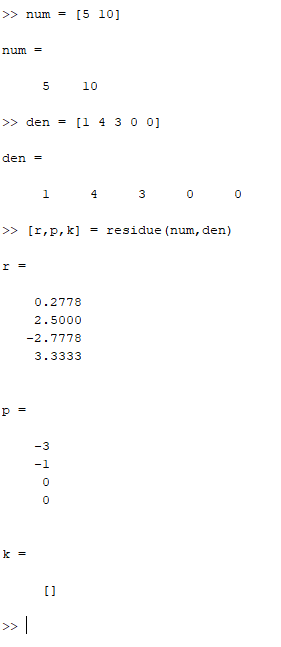
\includegraphics{figures/rpk.png}
    \caption{Output of residue(num, den), the $ r $ values are equivalent to $ A,B,C,D. $}
    \label{fig:fig1}
  \end{figure}

  Finally, the inverse laplace transform is,

  \begin{equation}
    f(t) = \frac{-25}{9} + \frac{10}{3}t + \frac{5}{2}e^{-t} + \frac{5}{18}e^{-3t}
  \end{equation}
  \section{}

  Given,

  \[
      F(s) = \frac{3s + 1}{s^4 + 3s^3 + 2s^2}
    .\]

  Factor the denominator to get the poles and zeroes,

  \begin{equation}
    F(s) = \frac{3s + 1}{s ^2 (s + 2)(s + 1)}
  \end{equation}

  \begin{align*}
    p &= 0,0,-2,-1 \\
    z &= -1/3
  \end{align*}

  Figure \ref{fig:fig2} shows the matlab commands used to check the values for $ p, z. $

  \begin{figure}
    \centering
    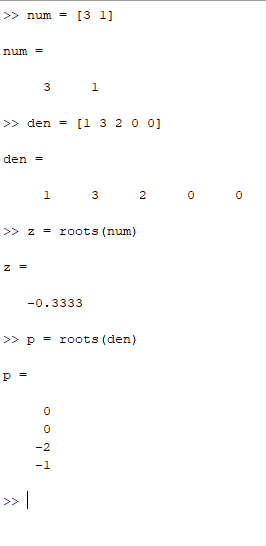
\includegraphics{figures/rootsandpoles.png}
    \caption{Matlab commands confirming values for $ p, z. $}
    \label{fig:fig2}
  \end{figure}

\end{document}
